\chapter{Inklusion-Exklusion}

  \begin{figure}[h]
    \centering
    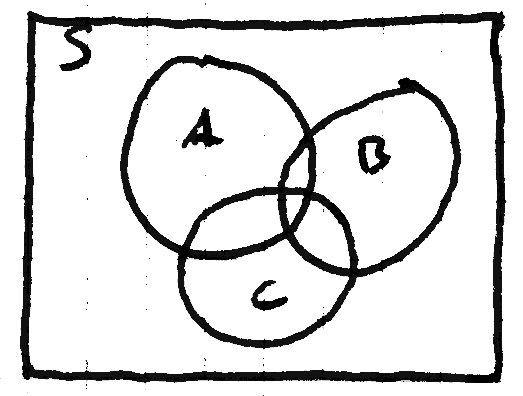
\includegraphics[width=.25\textwidth]{./Bilder/b03.jpg}
    % b01.jpg: 495x434 pixel, 72dpi, 17.46x15.31 cm, bb=0 0 495 434
  \end{figure}
  
  Gehe von einem Problem aus, bei es leicht ist zu zählen, welche Elemente aus dem Universum \(S\) die Eigenschaft \(A\) oder \(B\), \(A\) und \(B\), ... erfüllen; es aber schwer ist zu zählen, wie viele Elemente diese Eigenschaften nicht besitzen. Es ergibt sich jedoch der Zusammenhang
  
  \[ | \overline{A \cup B \cup C} | = |S| - ( |A| + |B| + |C| ) + ( |A \cap B| + |A \cap C| + |B \cap C| ) - ( | A \cap B \cap C | ). \]
  
  Sind \(N\) Objekte und eine Menge \(P = \{ P_1,\dots,P_n \}\) von Eigenschaften gegeben, bezeichnen wir für jedes \(S \subseteq P\) mit \(N(S)\) die Anzahl der Objekte, die (mindestens) die Eigenschaften in \(S\) erfüllen. Mit \(N(0)\) bezeichnen wir die Anzahl der Objekte, die keine der Eigenschaften erfüllen. Wir können oben skizzierte Formel dann verallgemeinern, es ergibt sich
  
  \begin{theorem} \label{satzInklSumme}
    \(N(0) = \sum_{S \subseteq P} (-1)^{|S|} N(S) = N(\emptyset) + \sum_i N(P_i) + \sum_{i \leq j} N(P_i, P_j) + ...\).
  \end{theorem}
  
  \begin{proof}
    Elemente des Universums, die keine der Eigenschaften besitzen, werden auf beiden Seiten der Gleichung einmal gezählt. Betrachte nun die Elemente, die genau die Eigenschaften \(S = \{ P_{i_1}, ..., P_{i_s}\}\), \(|S| = s\). Diese werden genau in den \(N(S')\) mit \(S' \subseteq S\) gezählt. Daraus folgt, dass diese Objekte zur rechten Seite der Gleichung jeweils \( \sum_{S' \subseteq S} (-1)^{|S'|} = \sum_{i=0}^s \binom{s}{i} \cdot (-1)^i = (-1 + 1)^s = 0\) beitragen. Objekte, die mindestens eine Eigenschaft besitzen, werden also auf der rechten Seite nicht gezählt.
  \end{proof}
  
  \begin{corollary}
    \(N(P) = \sum_{S \subseteq P} (-1)^{|S|}\overline{N}(S)\), wobei \(\overline{N}(S)\) die Anzahl der Objekte mit keiner der Eigenschaften in \(S\) ist.
  \end{corollary}
  
  \begin{proof}
    Es sei \(P'_i\) die Eigenschaft, dass ein Objekt die Eigenschaft \(P_i\) nicht besitzt. Es ist dann \(N'(0) = N(P)\) und \(N'(P'_1, ... P'_k) = \overline{N}(P_1,...,P_k)\). Es folgt die Behauptung.
  \end{proof}
  
\begin{section}{Gerichteter Hamiltonpfad}
  Wir betrachten nun das gerichtete Hamiltonpfadproblem. Gegeben sei ein gerichteter Graph \(G = (V,E)\) sowie Knoten \(s,t \in V\). Das gerichtete Hamiltonpfadproblem bezeichnet das Problem, ob ein einfacher \(s\)-\(t\)-Pfad existiert, der alle Knoten in \(V\) besucht. Dieses Problem ist NP-schwer. Brute force benötigt \(O^*(n^n)\) Zeit. Wir geben einen Algorithmus an, der \(O^*(2^n)\) Zeit und polynomiellen Speicherplatz benötigt.
  
  Möglich wäre eine Redukution auf TSP -- verbinde $t$ und $s$ durch eine Kante, suche eine kürzeste Rundtour, wobei zum vollständigen Graphen fehlende Kanten mit sehr hohem Gewicht eingefügt werden. Dies läuft zwar in $O^*(2^n)$ Zeit, braucht aber ebenfalls $O^*(2^n)$ Platz.
  
  \begin{theorem}
    Die Anzahl der \(s\)-\(t\)-Hamiltonpfade kann in \(O^*(2^n)\) Zeit und mit polynomiellen Speicherplatzverbrauch ermittelt werden.
  \end{theorem}
  
  \begin{proof}
    Wir verwenden das Inklusion-Exklusion-Prinzip. Als Objekte sehen wir alle \(s\)-\(t\)-Pfade der Länge \(n - 1\) an -- auch solche, die nicht einfach sind. Sei $V' \defNotion V \setminus \{s,t\}$. Die Eigenschaften \(v \in V'\) sind definiert als "`Pfad besucht den Knoten \(v\)"'. Also ergibt sich \(N(V')\) als die Anzahl der \(s\)-\(t\)-Hamiltonpfade. Zur Berechnung von \(N(V')\) bestimmen wir zunächst für \(W \subseteq V'\) jeweils \(\overline{N}(W)\), die Anzahl der \(s\)-\(t\)-Pfade der Länge \(n - 1\), die \(W\) vermeiden. 
    
    \[N(V') = \sum_{W \subseteq V'} (-1)^{|W|} \overline{N}(W)\]
    
    Dies erreichen wir durch dynamische Programmierung. Das Programm berechnet für ein festes \(W \subseteq V'\), ein \(k = 0,...,n-1\) und ein \(u \in V \setminus W\) die Anzahl der \(s\)-\(u\)-Pfade der Länge \(k\), die \(W\) vermeiden. Diese Zahl nennen wir \(\overline{N}(W,u,k)\). Es folgt \(\overline{N}(W,t,n-1) = \overline{N}(W)\). Die Berechnung erfolgt für \(k = 0\) durch
    \[
      \overline{N}(W,u,0) = 
      \begin{cases}
        1 & (u = s) \\
        0 & (\text{sonst})
      \end{cases}
    \]
    und für \(k > 0\) durch
    \[
      \overline{N}(W,u,k) = \sum_{vu \in E, v \notin W} \overline{N}(W,v,k-1)
    \]
    Die Laufzeit des dynamischen Programms für ein festes \(W\) ist \( O(n \cdot m) \) mit \(m = |E|\). Für den Speicher gilt:
    \[\overline{N}(\cdot,\cdot,\cdot) \leq 2^m \Rightarrow |\overline{N}(\cdot,\cdot,\cdot)| \leq m \text{ bits,}\]
    also insgesamt $O(n\cdot m)$.
    
    Zur Berechnung des Endergebnisses iterieren wir über alle \(W \subseteq V \setminus \{s,t\}\) und berechnen jeweils \( \overline{N}(w) \) mit dem oben angegebenen dynamischen Programm. Wir addieren den Wert des Ausdrucks \( (-1)^{|W|} \cdot \overline{N}(w) \) und erhalten \(N(V)\) als Wert dieser Summe. Die Gesamtlaufzeit ergibt sich damit als \(O(m \cdot n \cdot 2^n)\), der Gesamtspeicherbedarf als \(O(m \cdot n)\), da der Speicher wiederverwendet werden kann.
  \end{proof}
\end{section}
  
\begin{section}{Graphfärbung}
  Wir betrachten nun das Problem der Graph-Färbung. Als Eingabe sei ein Graph \(G = (V,E)\) gegeben. Eine \defNotion{zulässige Färbung} weißt jedem Knoten so einer Farbe zu, dass keine zwei benachbarten Knoten die selbe Farbe haben. Gesucht ist die minimale Anzahl an Farben, mit denen dies möglich ist. Brute force benötigt die Zeit \( O^*(n^n) \). Wir geben einen Algorithmus an, der \(O^*(2^n)\) Zeit und Speicherplatz benötigt.
  
  Wir nennen die Menge aller Knoten einer bestimmten Farbe eine \defNotion{Farbklasse}. Für korrekte Färbungen ist eine Farbklasse eine unabhängige Knotenmenge, daher können wir das Graphfärbungsproblem auch als Problem, die kleine Anzahl an unabhängigen Knotenmengen \(I_1,...,I_k\), die \(V\) partitionieren, formulieren. Dies ist verwand zum Set-Cover-Problem $(V, \mathcal{I})$, wobei \(\mathcal{I}\) die Menge aller unabhängigen Mengen in $G$ ist. Verallgemeinert betrachten wir daher Set-Cover-Instanzen $(U,S)$ (siehe Approximationsalgorithmen), bei denen $U$ explizit gegeben ist und $S$ in $O^*(2^{|U|})$ aufgezählt werden kann. 
  
  Wir nennen ein $S'$ ein \defNotion{$k$-Cover}, wenn $S' \subseteq S$, $\bigcup S' = U$ und $|S'| = k$. Wir entwerfen einen Algorithmus, der die Anzahl $c_k$ der \underline{geordneten $k$-Cover} $(S_1,\dots,S_k)$, $S_i \in S$, $\bigcup_{i=1}^k S_i = U$ ermittelt.
  
  \(W \subseteq U\) sei \(S[W]\) definiert als \( \{ S_i \in S : S_i \cap W = \emptyset \} \) sowie \(s[W] = |S[W]|\).
  
  \begin{lemma}
   Die Anzahl der geordneten $k$-Cover beträgt 
   \[c_k = \sum_{W \subseteq U} (-1)^{ |W| } s[W]^k\text{.}\]
  \end{lemma}

  \begin{proof}
    Wir betrachten die \(k\)-Tupel \( (S_1, ..., S_k) \) als Objekte und für \(v \in U\) den Ausdruck \(v \in \bigcup_{i=1}^k S_i\) als Eigenschaft, und wenden darauf die Inklusions- / Exklusionsformel an. Die Eigenschaft \(v \in U\) für ein \(k\)-Tupel gilt also nicht, wenn \(v \notin \cup_{i=1}^k S_i\). Ist ein \(W \subseteq U\) gegeben, so gelten alle Eigenschaften aus \(W\) nicht, wenn für alle \(v \in W\) stets \(v \notin \bigcup_i S_i\) gilt. Anders formuliert, muss für alle \(i\) der Schnitt \(S_i \cap W = \emptyset\) sein. Da es genau \(s[W]\) Mengen gibt, die \(W\) vermeinden, gibt es \(s[W]^k\) Möglichkeiten, ein \(k\)-Tupel aus Mengen zu bilden, die \(W\) vermeiden. Es ist damit \( \overline{N}[W] = s[W]^k\). Satz \ref{satzInklSumme} liefert dann \[c_k = N[U] = \sum_{W \subseteq U} (-1)^{ |W| } s[W]^k\] als Anzahl der Tupel, für die alle Eigenschaften \(v \in U\) gelten. Dies ist die Anzahl der Tupel, in denen für jedes \(v \in U\) gilt dass \(v \in \bigcup_i S_i\) ist.
  \end{proof}

  \begin{theorem}
    Die Anzahl \(c_k\) aller \(k\)-Cover kann in \(O^*(2^n) = O(2^n \cdot poly(n))\) berechnet werden. [vgl. 1.ÜB: $O(2^n \cdot poly(|S|,n))$]
  \end{theorem}

  \begin{proof}
    Es ist \(c_k = \sum_{W \subseteq U} (-1)^{ |W| } s[W]^k\). Zum Auswerten der Formel müssen alle Teilmengen \(W \subseteq U\) aufgezählt und jeweils \(s[W]\) berechnet werden. Dazu ordnen wir die Elemente von \(U\) durch \(U = \{u_1,...,u_n\}\) beliebig. Dann sei für alle \(W \subseteq U\)
    \[ g_i(W) = | \{ S_i \in S[W] : \{ u_1, ..., u_i \} \setminus W \subseteq S_i \} |. \]
    Dies ist die Anzahl der Mengen, die \(W\) vermeiden, und alle Elemente \(\{ u_1, ..., u_i \} \setminus W\) enthält.
    Mit dieser Definition gilt \(s[W] = g_0(W)\), denn \(g_0(W) = | \{ S_i \in S[W] : \emptyset \subseteq S \} | = | S[W] |\). Wir verwenden ein dynamisches Programm, das über \(i = n, ..., 0\) iteriert und zunächst
    \[
       g_n(W) =
       \begin{cases}
          1 & \text{ falls }U \setminus W \in S \\
          0 & \text{ sonst}
       \end{cases}
    \]
    berechnet. Für \(0 \leq i < n\) ist dann
    \[
      g_{i-1}(W) =
      \begin{cases}
         g_i(W) & \text{ falls }u_i \in W \\
         g_i(W \cup \{ u_i \}) + g_i(W) & \text{ falls }u_i \notin W
      \end{cases}
    \]
    Im Fall \(u_i \in W\) ändert sich durch den Ausschluss von \(W\) in der Definition von \(g_i\) nichts an der Bedingung, daher bleibt die Anzahl gleich. Im anderen Fall können zwei Fälle eintreten, deren Möglichkeiten addiert werden. \(g_i(W \cup \{ u_i \})\) erfasst die Elemente, die \(u_i\) vermeiden, während \(g_i(W)\) die Möglichkeiten enthält, die \(u_i\) enthalten. Für jede Menge \(W \subseteq S\) wird der Ausdruck \(g_i(W)\) \(n\)-mal ausgewertet, daher beträgt die Laufzeit \(O^*(2^n)\). Der Speicherverbrauch liegt bei \(O(2^n)\), wenn man zu jeder Zeit immer nur die vorhergehende Zeile in der dynamischen Tabelle speichert. Somit kann die Formel mit Hilfe von diesem Algorithmus in \(O(2^n)\) Speicher und Zeit ausgewertet werden.
  \end{proof}
  \begin{corollary}
   Graph-coloring kann in $O^ *(2^n)$ Zeit gelöst werden.
  \end{corollary}
  \begin{proof}
   Ermittle $c_k$ für alle $k = 1, \dots, n$ und bestimme das kleinste $k^*$, sodass $c_{k^*} > 0$. Verwende dazu die Instanz $(V,\mathcal{I})$.
  \end{proof}


\end{section}